\section{Modellierung}\label{sec:Modellierung}

Die erste Phase der aktiven Softwareentwicklung befasst sich mit den Fragen zum System. Dabei gilt es besonders darauf zu achten, das vermeintliche 'triviale' Aufgabenstellungen mit berücksichtigt werden und nicht etwa vernachlässigt oder vergessen werden.  In \prettyref{subsec:Objektorientierte Modellierung} wird näher auf die diese Problematik eingegangen. Dieses Problem tritt vor allem dann auf, wenn das System in einer späteren Phase des Projekts noch sinnvoll erweitert werden soll oder in Zukunft eine bestimmte Funktionalität verbessert werden muss.

Um dem Leser einen möglichst genauen Einblick in die Phasen der Modellierung geben zu können, ist der Aufbau dieses Abschnitts wie in \prettyref{subsec:Uber diese Ausarbeitung} bereits erwähnt, so gewählt, dass die einzelnen Schritte nach den verschiedenen Rollen des System gegliedert sind.

Im ersten \prettyref{subsec:Anforderungen an das System} sollen alle Anforderungen an das neue System und damit die Anforderungen an unsere Projektarbeit skizzenhaft aufgezeigt werden.
Im nächsten Schritt soll die Modellierung, und damit die ersten Überlegungen zum Design der Software, der gerade beschriebenen Anforderungen ausführlich besprochen werden.
Im darauffolgenden Abschnitt soll die \ac{OOM} angesprochen werden. Es zeigt wie mit Hilfe der \gls{Unified Modelling Language} (UML) das erste Design des System ensteht.  
Im \prettyref{subsec:Benutzerschnittstellen und Rollensystem} steht die Umsetzung des Systems und der verschiedenen Rollen im Vordergrund desweiteren zeigt es wie die Anforderungen umgesetzt sind.
Der \prettyref{subsec:Datenbankmodellierung} geht näher auf die Entwicklung des \ac{DB}-Systems zur Informationsverwaltung ein.
Der letzte Abschnitt im Teil der Modellierung ist unter \prettyref{subsec:Konfiguration der Laufzeitumgebung und des Server} zu finden und beschreibt die komplette Konfiguration von Server und Infrastruktur, also der kompletten Laufzeitumgebung, an der Schillerschule. 

\subsection{Anforderungen an das System}\label{subsec:Anforderungen an das System}

Außer den Problemen die mit dem alten Tool bestehen gibt es zusätzlich weitere neue Anforderungen an das System, die den Schulalltag und vor allem die Kurswahl und -verwaltung einfacher machen sollen.
Es werden dem Leser zunächst die Anforderungen an das neue Tool aufgezeigt um später Rückschlüsse auf die Funktionalität und die gesamte Umsetzung ziehen zu können.
An dieser Stelle wird angemerkt, dass es sich hierbei um die originalen Anforderungsspezifikationen vor Projektbeginn handelt.

\textbf{Allgemeine Systemanforderungen}

\begin{itemize}
  \item webbasierte Zugang zum System über das \ac{WWW} und im Intranet
  \item Rollenunterstützung um Berechtigungen zu unterscheidende
  \item Benutzerrelevante Daten sollen angezeigt werden und bearbeitet werden können
\end{itemize}

\textbf{Schüler}

\begin{itemize}
  \item Wahl von Kursen
  \item Einsicht in Leistungsübersicht:
    \begin{itemize}
      \item Protfoliofunktion 
      \item Druck- und Exportfunktion
    \end{itemize}
\end{itemize}

\textbf{Kurslehrer}

\begin{itemize}
  \item Einsicht der Teilnehmerlisten von Kursen
  \begin{itemize}
    \item Druck- und Exportfunktion
  \end{itemize}
  \item Eingabe von Leistungsnachweisen der Kurse
  \begin{itemize}
    \item Druck- und Exportfunktion
  \end{itemize}
\end{itemize}

\textbf{Klassenlehrer}

\begin{itemize}
  \item Einsicht einer Klassenübersicht
  \begin{itemize}
    \item Druck- und Exportfunktion 
  \end{itemize}
  \item Eingabe von Leistungsnachweisen
  \begin{itemize}
    \item bearbeiten des Portfolios der einzelnen Schüler in der Klasse
    \item Druck und Exportfunktion des Portfolios, der Klassenliste und alle Schüler mit ihren gewählten Kursen in der Klasse
  \end{itemize}
\end{itemize}
 
\textbf{Admin}

\begin{itemize}
  \item Erstellung/Verwaltung des Kursangebots
  \item Erstellung/Verwaltung der Klassenlisten
  \item Erstellung/Verwaltung der Leistungsnachweise
  \begin{itemize}
    \item Druck- und Exportfunktion
  \end{itemize}
\end{itemize}

Aus den ersten Überlegungen entstand folgende Mindmap welche unter \prettyref{fig:Projekt_Mindmap} zu sehen ist.

An erster Stelle befindet sich das System mit dessen Laufzeitkomponenten und Eigenschaften. Der zweite Punkt beinhaltet Schlagwörter die auf die Interaktionsmöglichkeiten des Systems zurückgehen. Schnell wurde klar, dass es sich um ein sehr dynamisches und stetig veränderndes System handeln muss. Außerdem mussten alle Anwendungsfälle des Systems möglichst zu Projektbeginn abgedeckt und durchdacht werden um später irreversible Änderungen zu vermeiden. Auf diesen Punkt wird allerdings in \prettyref{subsec:Objektorientierte Modellierung} noch näher eingegangen.

% KuWaSys MindMap
\begin{figure}[H]
\centering\begin{tikzpicture}[mindmap,
  level 1 concept/.append style={level distance=130,sibling angle=30},
  extra concept/.append style={color=blue!50,text=black}]

\begin{scope}[mindmap, concept color=orange, text=white]
\node [concept]at (-2,1) {System 'KuWaSys'}[clockwise from=-5]
    child [grow=10] {node [concept] (S) {Rollensystem}}
    child {node [concept] (L) {Kurssystem}}
    child[grow=230] {node [concept] (L) {Webapp}};
\end{scope}
\begin{scope}[mindmap, concept color=blue!70!black,text=white]
\node [concept] at (4.5,-6) {Interaktion}
      child [grow=155, level distance=120]{node [concept] (cr) {erstellen}}
      child [grow=90] {node [concept] (ch) {wählen}}
      child [grow=200] {node [concept] (un) {abwählen}}
      child [grow=15] {node [concept] (un) {verwalten}};
\end{scope}
\end{tikzpicture}
\caption[\textbf{Projekt Mindmap}]{Projekt Mindmap}
\label{fig:Projekt_Mindmap}
\end{figure}

\subsection{Objektorientierte Modellierung}\label{subsec:Objektorientierte Modellierung}

Wie schon in \prettyref{sec:Modellierung} angesprochen, soll nun die \ac{OOM} zur Sprache kommen.

Zu Beginn sollen die von uns erstellten Anwendungsfälle, die sich aufgrund genauerer Analyse der Anforderungsspezifikation des Systems ergeben haben, näher erläutert werden.
Hierzu wurde die \ac{UML}, wie schon oben beschrieben, mit Hilfe eines \ac{UC-Diagramm}s, verwendet.

\subsubsection{Use-Case Modell}

% Use Case Diagramm
\begin{figure}[H]
 \begin{center}
   \includegraphics[scale=0.5]{img/UseCaseModel_kuwasys20.png}
 \end{center}
 \caption[\textbf{Use Case Diagram: Rollensystem}]{Use Case Diagramm: Rollensystem}
 \label{fig:UML_UC_kuwasys20}
\end{figure}

'Ein \ac{UC} beschreibt die Funktionalität des Softwaresystems, die ein Akteur ausführen muss, um ein gewünschtes Ergebnis zu erhalten oder um ein Ziel zu erreichen. \ac{UC}s sollen es ermöglichen, mit dem zukünftigen Benutzer über die Funktionalität des Softwaresystems zu sprechen, ohne sich gleich in Details zu verlieren.' (\iz{Heide Balzert}{Informatikerin, die sich vor allem mit Fragen zum Thema Softwareengineering und -design beschäftigt. Derzeit ist sie Dozentin an der Fachhochschule Dortmund.}, \cite{BalzertH-UML2}, 28).

Zusammenfassend bedeutet dies, dass ein \ac{UC-Diagramm} immer dann sinnvoll ist wenn die Interaktionsmöglichkeit eines Systems, basierend auf verschiedene Aktueren, aufgezeigt werden soll. Die Akteure (dargestellt als 'Strichmännchen') im Diagramm, entsprechen genau denen, die später vom Rollensystem unterstützt werden sollen. Die Ellipsen zeigen die verschiedenen Anwendungsfälle die im System existieren. In einem so allgemeinen \ac{UC-Diagramm} wird absichtlich auf kleinste Details verzichtet. So bedeutet zum Beispiel der \ac{UC} 'Klasse verwalten' sowohl das Bearbeiten einer Klasse als auch das Vergeben von Noten oder andere klassenadministrative Aufwendungen.

Die gestrichelten Pfeile mit der Beschriftung '\texttt{$<<$include$>>$}' bezeichnen Anwendungsfälle in denen der \ac{UC}, auf welchen der Pfeil zeigt, implizit vorhanden ist wenn der \ac{UC}, von dem der Pfeil ausgeht, im System vorhanden ist. Das bedeutet wenn der \ac{UC} 'User anlegen' also vorhanden ist, auch die \ac{UC}s 'Schüler importieren' oder 'User verwalten' verwendet werden können. Ein erster \ac{UC} muss also immer erfolgen während ein zweiter (oder noch mehr) optional ausgeführt werden können.

Im Gegensatz hierzu bedeutet der gestrichelte Pfeil mit der Beschriftung '\texttt{$<<$extend$>>$}' von dem der Pfeil ausgeht, dass dieser \ac{UC} nur dann im System überhaupt vorhanden ist, wenn der \ac{UC} auf welchen der Pfeil zeigt im System vorhanden ist. Der \ac{UC} 'Kurs abwählen' ist also nur dann vorhanden wenn der \ac{UC} 'Kurs wählen' im System ausgeführt wurde. Der erste \ac{UC} wird durch den zweiten also erweitert.

\subsubsection{Statisches Analysemodell}

Im nächsten Schritt unserer Modellierung ist das statische Analysemodell, unter \prettyref{fig:UML_SA_kuwasys20} zu sehen, entworfen worden. Es stellt erste Überlegungen der Softwarearchitektur, mit konkreten Objekten inklusiver ihrer Attribute, dar und bildet ebenfalls die Beziehungen von Objekten zueinander ab. Genau genommen handelt es sich hierbei um ein 'abgespecktes' Klassendiagramm, in welchem die grobe Softwarestruktur erkennbar sein soll.

Die rechteckigen Formen stellen Klassen dar, die oben als Beschriftung ihren Namen tragen, unten die Attribute die zu ihr gehören. Die einfachen Linien sind Assoziationen zwischen den Klassen und können als Beziehungen interpretiert werden. Sie tragen einen Rollennamen und eine Multiplizität, um nachvollziehen zu können um wieviele Objekte einer Klasse es sich später mindestens und maximal handelt.
Die Rechtecke mit der Beschriftung \texttt{$<<$dataType$>>$ + String} stellen selbstdefinierte Datentypen dar.
Die Besonderheit in diesem Diagramm ist die Komposition (Assoziation mit einseitg schwarzer Raute). Sie sagt aus dass die Beziehung zwischen zwei Klassen einer starke Form der Aggregation entspricht. Die Teilklasse (Notenliste) kann also nur bestehen, solange die Aggregatklasse (Kurs) auch besteht. Würde, angewendet auf dieses Beispiel, ein Kurs gelöscht werden, würde auch der dazugehörige Notenlisteneintrag gelöscht werden. (\cite{BalzertH_UML2}, 18)

In unserem Projekt entstanden zum Zeitpunkt des Softwareentwurfs 3 Klassen, die später für eine Interaktion mit dem System benötigt werden und dementsprechend die wichtigsten Objekte abbilden. Die Klasse für die Notenübersicht und für Kurse. Die verschiedenen Rollen wurden als Unterklassen der Klasse 'User' modelliert. Einzelne Datentypen, so bspw. für Daten zur Zeiterfassung (Datum) und zur Definition einzelner konstanter Strings (Name), wie die Rollen, wurden zur Vereinfachung vorgesehen.
Die Rollennamen sowie die Multiplizitäten der Assoziationen dürften selbsterklärend sein.
In Abschnitt \prettyref{sec:Implementierung} wird später näher auf die restlichen Handler- und Helper-Klassen eingegangen

% Statisches Analyse Diagramm
\begin{figure}[H]
 \begin{center}
   \includegraphics[scale=0.7]{img/StaticClassModel_kuwasys20.png}
 \end{center}
 \caption[\textbf{Statisches Analysemodell}]{Statisches Analysemodell}
 \label{fig:UML_SA_kuwasys20}
\end{figure}

\subsection{Benutzerschnittstellen und Rollensystem}\label{subsec:Benutzerschnittstellen und Rollensystem}

Das Kurswahlsystem der Schillerschule soll, laut Anforderungen, webbasiert mit Hilfe von verschiedenen Rollen konfiguriert und benutzt werden können.
Das System muss hierzu simultane Interaktionen, eines jeden Rollentyps, mit dem System zulassen. 

Per Aufgabendefinition liegen die vier Rollen, wie in \prettyref{subsec:Anforderungen an das System} bereits behandelt, zugrunde:

\begin{itemize}
  \item Schüler
  \item Kurslehrer
  \item Klassenlehrer
  \item Admin
\end{itemize}

Anhand der bereits vorgestellten \ac{OOM} sind, vor der Implementierung des Systems, die Rollenrechte und -richtlinien welche in den folgenden drei Unterabschnitten genaue beschrieben werden, modelliert worden.

\subsubsection{Die Rolle der Schüler}

Bei der Rolle der Schüler handelt es sich um die einfachste des Systems. 
Sie hat die wenigsten Rechte und kann hauptsächlich nur passiv, Ausnahme bildet hier die Kurswahl selbst, mit dem System interagieren.
Die Schüler welche das Kurswahlsystem erstmalig benutzen, befinden sich in der 7. Klasse. Jeder Schüler wird bis zum Abschluss der 9. Klasse das System benutzen.
Ein Schüler soll selbstständig seine Kurswahl für das jeweilige bevorstehende Tertial eines Schuljahres treffen können, dabei müssen bestimmte Abhängigkeiten eingehalten werden:

\begin{enumerate}
  \item 6 unterschiedliche Kurse pro Tertial
  \item 18 Kurse im Schuljahr
  \item 54 Kurse bis zur Vollendung des 9. Schuljahres
\end{enumerate}

\subsubsection{Die Rolle der Lehrer}

Der Rolle des Lehrers ist hingegen schon weitaus mehr Verantwortung auferlegt.
Das System unserer Webandwendung unterscheidet allerdings zwischen zwei verschiedenen Arten von Lehrern grundsätzlich nicht aufgrund einer Rollendefinition. 
Die Befugnis eines Lehrers sind lediglich abhängig von Werten die in der \ac{DB} gespeichert werden. 
Ein Klassenlehrer wird nur dann ein Klassenlehrer wenn für ihn eine Abhängigkeit zu einer Klasse besteht. 
Erst dann kann er die Funktionen, die einenm Klassenlehrer zu Verfügung stehen, nutzen.
Ein Klassenlehrer muss auf die ihm zugerordnete Klasse zugreifen und alle Kurse eines jeden Schülers einsehen können.

Das gleiche Prinzip gilt für Kurslehrer. 
Beim anlegen eines Kurses (eine Funktion die jedem Lehrer generell zur Verfügung steht) wird dieser Kurs dem Lehrer fest zugeordnet und wird somit zum Mitverantwortlichen der Kursverwaltung. 
Der Kurslehrer muss ebenfalls die Schüller einsehen können die sich in seinem Kurs befinden. Allerdings kann er nur ein Protokoll und eine Notenliste für Schüler in seinem Kurs führen.

In Abhängigkeit zur administrativen Systemverwaltung, auf die im nächsten Teil-Block eingegangen wird, hat der Lehrer nun die Rechte seine Kurse zu verwalten.

Zur Vereinfachung der Handhabung des Systems ist bereits an diesem Punkt der Modellierung an ein internes Protokollierungssystem gedacht worden. 
Es soll später die Kommunikation von Kurslehrern mit Klassenlehrern sowie die Kommunikation von Lehrern mit Schülern vereinfachen.
Im Rahmen unserer Projektarbeit wurde allerdings eine solche Funktionalität im System nicht implementiert.

\subsubsection{Die administrative Rolle des Systems}

Die administrativen Rechte des kompletten Systems stehen selbstverständlich nur dem Administrator zur Verfügung. Die Hauptaufgabe dieser Rolle im System ist es neue User ins System aufzunhemen und diese gegebenfalls zu Bearbeiten.
Das gilt für das Hinzufügen und Bearbeiten von Schülern und Lehrern gleichermaßen, beide Rollen haben also nicht die Möglichkeit sich selbst zu Verwalten.

Darüber hinaus verwaltet der Admin den Status des Systems, das aktuelle Schuljar und die dazughörigen Tertiale. Außerdem ist er der Hauptverantwortliche der Kursverwaltung.
Bevor ein Kurs stattfinden kann muss der Admin den Kurs aktivieren und für die Kurswahl zulassen. Eventuell müssen von ihm bestimmte Attribute eines Kurs noch angepasst werden können.
Ein Admin kann außerdem Fächerverbünde erstellen, bearbeiten und erstellte Kurse einem Fächerverbund zuordnen.

\subsubsection{Funktionalität des Systems}

Die Einteilung eines kompletten Schuljahrs geschieht jeweils in Tertiale. Dies kann grafisch in \prettyref{fig:Schuljahreinteilung} nachvollzogen werden. 

%%
% Schuljahreinteilung
\begin{figure}[h]
\begin{center}

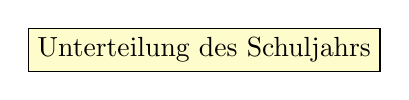
\begin{tikzpicture}
    \node[draw=black, fill=yellow!20!] at (-2.5,5) {Unterteilung des Schuljahrs};
    \pie{33.3/Tertial 1, 33.3/Tertial 2, 33.3/Tertial 3}
\end{tikzpicture}

\end{center}
\caption[\textbf{Einteilung des Schuljahrs}]{Einteilung des Schuljahrs}
\label{fig:Schuljahreinteilung}
\end{figure}

Es war also nötig im administrativen Bereich des Systems eine Funktionalität vorzusehen, die es dem Admin ermöglicht das Schuljahr 'weiterzuschieben' und das entsprechende Tertial zu zu aktivieren.
Diese Verwaltungstätigkeit ist unumgänglich mit der Kurswahl verknüpft und muss für jede neu angepasst werden. 
Entscheidungen die hier während der Modellierung getroffen wurden, wurden im Hinblick auf eine möglichst einfaches \ac{UI} getroffen.

Jeder Kurs, der gewählt werden kann, gehört einem übergeordnetem Fächerverbund an, wie in \prettyref{fig:KursFaecherverbund} zu sehen ist.
Allerdings gibt es noch weitere Eigenschaften die Kurse erfüllen können. Ein Kurs kann ein Religionskurs sein, welcher für eine bestimmte Konfession ausgerichtet ist oder ein Sportkurs.
Ferner müssen Kurse als Pflichtkurse signifiziert werden können.
Aufgrund der Fülle an Informationen die verarbeitet werden müssen, war es in der Phase der Modellierung ebenfalls sehr wichtig die Datenstrukturen und deren Abhängigkeiten möglichst einfach zu halten, um in der späteren Implementierungsphase eine unkomplizierte Benutzerschnittstelle entwicklen zu können. 

Außer den beiden vorgestellten Datenverarbeitungen existieren selbstverständlich noch weitere, die vor allem im Sinne der Übersichtlichkeit des System  zum Tragen kommen. 
Dabei handelt es sich allerdings um Daten, die dynamisch während der Laufzeit erzeugt werden.
Im Gegensatz zu den dynamisch generierten Daten während der Laufzeit des Systems ist für alle anderen Daten zur Informationsverarbeitung eine Speicherung in einer Datenbank unabdingbar.
Im folgenden Unterabschnitt soll deshalb näher auf die Modellierung und Umsetzung des verwendeten Informationssystems eingegangen werden.

\subsection{Datenbankmodellierung}\label{subsec:Datenbankmodellierung}

Für die \ac{DB}-Modellierung wurde als erstes ein \ac{ER-Modell} skizziert, welches die Abhängigkeiten und Beziehungen zueinander verdeutlichen soll. Dieses ist in \prettyref{subsec:ERModell} abgebildet. Anschließend wurde das gesamte \ac{ER-Modell} in ein relationales Modell transformiert.
Mit dem entstandenen Relationalen Modell, welche in \prettyref{subsec:RelModell} dokumentiert ist, konnte anschließend auf dem Server die \ac{DB} inklusive der nötigen Tabellen erstellt werden.

\subsubsection{Entity-Relationship Modell}\label{subsec:ERModell}

Die \prettyref{fig:ERModell} zeigt das oben erwähnte \ac{ER-Modell} nach \iz{Peter Pin-Shan Chen}{Informatiker, der 1976 das ER-Modell entwickelte. Er gilt heute als Pioneer der \ac{OOM}.} (\cite{ChenPe}, 3 ff. bzw. \cite{VossenG-DDD}, 60 ff.).

\textbf{Aufbau des \ac{ER-Modell}s:}

Bei den blauen Rechtecken handelt es sich in diesem Modell um sogenannte Entities (Entity-Typen), die sind Dinge die in der \ac{DB} als solche abgebildet werden sollen. Sie stellen eine eigene Tabelle dar. Die gelben Ellipsen die diese umgeben, sind die Attribute (Attribut-Typen) der Entities, sie veranschaulichen die Daten welche Entities enthalten (können).
Die roten Rauten bezeichnen Beziehungen (Beziehungs-Typen) die zwischen Entities herrschen.

Das grüne Rechteck ist ein Spezialfall des 'Kurs'-Entities. Es wird als eigene Tabelle in der \ac{DB} dargestellt, ist im weitesten Sinne allerdings einer Aversion des 'Konfessions'-Attribut des 'Kurs'-Entities. Denkt man in diesem Fall an die \ac{UML}, so wäre an dieser Stelle wohl eine 'Enumeration' als eigener Datentype in Frage gekommen (\cite{BalzertH_UML2}, 10 - 11).

\tikzstyle{every entity} = [top color=white, bottom color=blue!30, draw=blue!50!black!100, drop shadow]
\tikzstyle{every weak entity} = [drop shadow={shadow xshift=.7ex, shadow yshift=-.7ex}]
\tikzstyle{every attribute} = [top color=white, bottom color=yellow!20, draw=yellow, node distance=1cm, drop shadow]
\tikzstyle{every relationship} = [top color=white, bottom color=red!20, draw=red!50!black!100, drop shadow]
\tikzstyle{every isa} = [top color=white, bottom color=green!20, draw=green!50!black!100, drop shadow]
\begin{center}
\begin{figure}[H]

\scalebox{.7}{
\begin{tikzpicture}[node distance=1.5cm, every edge/.style={link}]

%% USER
\node[entity] (usr) {Users};
\node[attribute] (usrvname) [above=2.5cm of usr] {VName} edge (usr);
\node[attribute] (usrnname) [above right=3cm of usr] {NName} edge (usr);
\node[attribute] (geb) [above left=3cm of usr] {Geburtsdatum} edge (usr);
\node[attribute] (usrkonf) [above left=of usr] {Konfession} edge (usr);
\node[attribute] (usrklasse) [above=of usr] {Klasse} edge (usr);
\node[attribute] (usrusername) [above right=of usr] {\key{Username}} edge (usr);
\node[attribute] (usrpassword) [right=of usr] {Passwort} edge (usr);
\node[attribute] (usrid) [below=0.3cm of usr] {\key{UserID}} edge (usr);

%% REL "hat"
\node[relationship] (hat) [left=1.5cm of usr] {hat} edge (usr);

%% REL "eingetragen"
\node[relationship] (eingetragen) [below left =3cm of usr] {eingetragen} edge (usr);
%
%% ROLLE
\node[entity] (rolle) [left=1cm of hat] {Rolle} edge (hat);
\node[attribute] (rollename) [left=of rolle] {\key{Username}} edge (rolle);
\node[attribute] (rolleusrnname) [above left=of rolle] {Rolle} edge (rolle);

%% REL "besucht"
\node[relationship] (besucht) [below right=of usr] {besucht} edge (usr);

%% KURS
\node[entity] (kurs) [below right=1cm of besucht] {Kurs} edge (besucht);
\node[entity, top color=white, bottom color=green!30, draw=green!50!black!100, drop shadow] (kurskonf) [above=1.5cm of kurs] {Kurskonfession} edge (kurs);
\node[attribute] (termin) [above right =.2cm of kurskonf] {Termin} edge (kurs);
\node[attribute] (kursl) [right =.2cm of kurskonf] {Kurslehrer} edge (kurs);
\node[attribute] (teilm) [above right=0.2cm of kurs] {Teilnehmerzahl} edge (kurs);
\node[attribute] (kursid) [left=0.2cm of kurs] {\key{KursID}} edge (kurs);
\node[attribute] (faecher) [right=0.2cm of kurs] {Fächerverbund} edge (kurs);
\node[attribute] (flags) [below=2.5cm of kurs] {Sportkurs} edge (kurs);
\node[attribute] (flag3) [below=2.2cm of faecher] {Pflicht} edge (kurs);
\node[attribute] (tertial) [below left=.2cm of flag3] {Tertial} edge (kurs);
\node[attribute] (flag2) [below=1.2cm of faecher] {Konfession} edge (kurs);
\node[attribute] (bemerk) [below=of kurs] {Beschreibung} edge (kurs);
\node[attribute] (kursname) [below right=0.2cm of kurs] {Kursname} edge (kurs);

%% REL "enthält"
\node[relationship] (enthalten) [below left =of kurs] {enthalten} edge (kurs);

%% NOTENLISTE
\node[entity] (notenliste) [below right=2cm of eingetragen] {Notenliste} edge (enthalten) edge (eingetragen);
\node[attribute] (note) [below left=1cm of notenliste] {Note} edge (notenliste);
\node[attribute] (usrkonf) [above =of notenliste] {Bemerkung} edge (notenliste);
\node[attribute] (usrvname) [below=of notenliste] {\key{KursID}} edge (notenliste);
\node[attribute] (usrnname) [left=of notenliste] {\key{UserID}} edge (notenliste);
\node[attribute] (listid) [below right=1.2cm of notenliste] {\key{ListenID}} edge (notenliste);

%% SYSTEM
\node[entity] (system) [below=5cm of notenliste] {System};
\node[attribute] (schuljahr) [below=of system] {Schuljahr} edge (system);
\node[attribute] (tertial) [left=of system] {Tertial} edge (system);
\node[attribute] (wochd) [below left= of system] {Phase} edge (system);
\end{tikzpicture}
}
\caption[\textbf{Entity-Relationship Modell}]{Entity-Relationship Modell}
\label{fig:ERModell}
\end{figure}
\end{center}

\textbf{Interpretation des \ac{ER-Modell}s:}

Um die Interpretation, also den Gedankengang der \ac{DB}-Modellierung, zu verdeutlichen macht es Sinn, die Beziehungen genau auszuformulieren.
Dabei werden alle Beziehungen zu jedem Entity betrachtet, begonnen mit dem Entity.
Zusätzlich sollen die Multiplizitäten mit einfließen, um die Abhängigkeiten zu verdeutlichen und um die Transformation in ein Datenbankmodell zu erleichtern.

Die Schreibweise dieser Multiplizitäten ist wie folgt definiert:

Sei $E_{A}$ das erste und $E_{B}$ das zweite Entity.
Die Beziehung beider Entities ist definiert als $R_{AB}$. 
Die erste Multipliziät $(0,N)$ gibt Auskunft über die Häufigkeit von $E_{A}$ in der geltenden Beziehung zu $E_{B}$.
Die zweite $(1;M)$ über die Häufigkeit von $E_{B}$ zu $E_{A}$.

Man kann also schreiben:

\begin{center}
$E_{A}$ ist $(0;N)$ in Beziehung $R_{AB}$ zu $E_{B}$

oder

$E_{B}$ ist $(1;M)$ in Beziehung $R_{AB}$ zu $E_{A}$
\end{center}

Wobei die erste Zahl bei der Angabe der Multiplizität, also die vor dem Semikolon (';') für die minimalste, die zweite Zahl für die maximalste Gültigkeit unter der bestendenen Bedingung steht.

Begonnen werden soll die genauere Betrachtungsweise mit dem Entity 'User':

\begin{enumerate}
  \item User - Rolle (beidseitig):	
    \begin{itemize}
      \item einem User ist genau $(1;1)$ Rolle zugeteilt
      \item einer Rolle hingegen können $(0;N)$ User zugeteilt sein
    \end{itemize}

  \item User - Kurs
    \begin{itemize}
      \item ein Schüler wählt $(0;N)$ viele Kurse
      \item ein Lehrer erstellt/verwaltet $(0;M)$ viele Kurse
    \end{itemize}
  
  \item User - Notenliste:
    \begin{itemize}
      \item ein Schüler hat $(1;1)$ Eintrag in der Notenliste für jeweils einen fest zugeordneten Kurs (Vrgl. Kurs - Notenliste)
    \end{itemize}

\end{enumerate}

Konkretisieren wir nun das Entity 'Kurs':

\begin{enumerate}
  \item Kurs - Notenliste:
  \begin{itemize}
    \item ein Kurs besitzt genau $(1;1)$ Eintrag pro Kurs in der Notenliste für einen Schüler (Vrgl. User - Notenliste)
  \end{itemize}
  
  \item Kurs - Kurskonfession	
    \begin{itemize}
      \item ein Kurs hat genau $(0;1)$ Konfessionszugehörigkeit
    \end{itemize}

  \item Kurs - User	
    \begin{itemize}
      \item ein Kurs wird von $(0;N)$ vielen Schülern gewählt
      \item ein Kurs wird immer genau $(1;1)$ Lehrern zugeteilt
    \end{itemize}
\end{enumerate}

Für das letzte Entity der Dreier-Beziehung 'Notenliste' gelten lediglich die bereits beschriebenen Abhängigkeiten und Beziehungsverhältnisse. 
Zur Verdeutlichung sollen diese jedoch nochmals aufgeführt werden.

\begin{enumerate}
  \item Notenliste - User:
  \begin{itemize}
    \item eine Notenliste hat im Bezug auf genau einen Kurs $(0;N)$ Einträge für einen User
  \end{itemize}
  
  \item Notenliste - Kurs:
  \begin{itemize}
    \item Ein Schüler wählt $(1;N)$ viele Kurse, ein Kurs wird von $(1;N)$ vielen Schülern besucht/gewählt.
  \end{itemize}
  
\end{enumerate}

Das Entity 'System' besitzt keine Beziehungen innerhalb der Datenbank, weshalb auf eine ausführliche Interpretation verzichtet werden kann.
Die Darstellung dieses Entities wird innerhalb der \ac{DB} sowieso über eine eigene Tabelle umgesetzt.

Der nächste Schritt ist nun die Transformation von \ac{ER-Modell} in das Relationale \ac{DB}-Modell.

\subsubsection{Relationales Modell}\label{subsec:RelModell}

Bei der Beschreibung des Relationalen Modells der KuWaSys-\ac{DB} ist das Hauptaugenmerk auf die komplette Datenverarbeitung gelegt, also vor allem auch Implementierungen für Vorgänge die für den Benutzer des Systems nicht unmittelbar zu sehen sind.
Daten die für die Oberfläche und die einzelnen Benutzerschnittstellen eine tragende Rolle spielen sollen unter (Abschnitt Benutzerschnittstellen) gesondert behandelt werden und werden im Laufe dieses Kapitels nur kurz angesprochen.

Die Vorüberlegungen zur Transformation von mehrwertigen Attributen von Entities sind bereits abgeschlossen.
Prinzipiell kann man mit der Transformation, wie folgt vorgehen (\cite{VossenG-DDD}, 104 ff.):

\begin{enumerate}
 \item Jedes Entity wird in eine relationale Form gebracht
 \item Jeder Beziehungs-Typ ebenfalls, es sei denn:
 \begin{itemize}
  \item es handelt sich um eine zweistellige $1:1$-Beziehung
  \item es handelt sich hierbei um eine $1:N$-Beziehung
 \end{itemize}
\end{enumerate}

Die Beschreibung $1:1$- bzw $1:N$-Beziehung bedeutet in diesem Fall allerdings nicht wie zuvor, ein Minimum auf der linken und das Maximum auf der rechten Seite. 
Hierbei werden nur noch die maximalen Werte der beiden Multiplizitätsangaben berücksichtigt. Dies gilt analog für alle Angaben der Multiplizitäten.

Sollte bei der Transformation $Punkt$ $2)$ eine Rolle spielen, müssen Attribute in bereits bestehende Relationsschemata aufgenommen werden. Folgende Regeln treten dann in Kraft:
\begin{enumerate}
 \item Zweistellige $1:1$-Beziehung
 \begin{itemize}
  \item ein Entity stellt selbst ein Relationsschema dar
  \item Attribute des zweiten Entities werden ebenfalls in dieselbe Tabelle gespeichert
 \end{itemize}
 \item Zweistellige $1:N$-Beziehung
 \begin{itemize}
  \item ein Entity stellt ein eigenes Relationsschema dar
  \item erste Möglichkeit: die Attribute des Entities welches die maximale Multiplizität von $1$ aufweist wird hingegen dem Realtionsschema mit der maximalen Multiplizität von $N$ in Form von Fremdschlüsseln zugeschrieben
  \item zweite Möglichkeit: es wird ein eigenes Relationsschema für die Beziehung der beiden Entities angelegt. Dieses neu entstande Schema erhält dann Attribute, welche widerum Fremdschlüssel der beiden anderen Entities sind
 \end{itemize}
\end{enumerate}

Die Transformation vom \ac{ER-Modell} ins Relationale Modell (zur bildhaften Darstellung ist die Kopfzeile der dazugehörigen Tabelle auch gezeigt) sieht im Falle des Kurswahlsystems folgendermaßen aus:

\textbf{Users} = \{( \underline{id:serial}, nachname:character, vorname:character, geburtstag:character, konfession:character, klasse:character, \underline{username:character}, passwort:character )\}

% User-Tabelle
\begin{table}[H]
\begin{center}
	\begin{tabular}{|c|c|c|c|c|c|c|c|}\hline
		\textbf{\underline{ID}} & \textbf{NName} & \textbf{VName} & \textbf{Geb} & \textbf{Konf} & \textbf{Klasse} & \textbf{\underline{Username}} & \textbf{Passwort} \\ \hline
		\vdots & \vdots & \vdots & \vdots & \vdots & \vdots & \vdots & \vdots \\
	\end{tabular}
	\caption{Kopfzeile der User-Tabelle}
\end{center}
\end{table}

\textbf{Kurs} = \{( \underline{id:serial}, name:character, kurslehrer:integer, faecherverbund:character, termin:integer, beschreibung:character, schuljahr:integer, tertial:integer, 
teilnehmerzahl:integer, pflichtkurs:boolean, sport:boolean )\}

% Kurs-Tabelle
\begin{table}[H]
\begin{center}
	\begin{tabular}{|c|c|c|c|c|c}\hline
		\textbf{\underline{ID}} & \textbf{Name} & \textbf{Kurslehrer} & \textbf{Faecherverbund} & \textbf{Termin} & \dots \\ \hline
		\vdots & \vdots & \vdots & \vdots & \vdots & \dots \\
	\end{tabular}
	\caption{Kopfzeile der Kurs-Tabelle  (unvollständig)}
\end{center}
\end{table}

\textbf{Kurs-Konfessionen} = \{( \underline{religionid:integer}, konfession:character )\} 
 
% Kurs-Konfession-Tabelle
\begin{table}[H]
\begin{center}
	\begin{tabular}{|c|c|}\hline
		\textbf{\underline{ReligionID}} & \textbf{Konfession} \\ \hline
		\vdots & \vdots \\
	\end{tabular}
	\caption{Kopfzeile der Kurs-Konfessions-Tabelle}
\end{center}
\end{table}

\textbf{Notenliste} = \{( \underline{id:serial}, note:integer, bemerkung:character, userid:integer, kursid:integer, jahr:integer, tertial:integer )\}

% Notenliste-Tabelle
\begin{table}[H]
\begin{center}
	\begin{tabular}{|c|c|c|c|c|c|c|}\hline
		\textbf{\underline{ID}} & \textbf{Note} & \textbf{Bemerkung} & \textbf{UserID} & \textbf{KursID} & \textbf{Jahr} & \textbf{Tertial}\\ \hline
		\vdots & \vdots & \vdots & \vdots & \vdots & \vdots & \vdots  \\
	\end{tabular}
	\caption{Kopfzeile der Notenlisten-Tabelle}
\end{center}
\end{table}

\textbf{Rolle} = \{( \underline{username:character}, rolle:character )\}

% Rollen-Tabelle
\begin{table}[H]
\begin{center}
	\begin{tabular}{|c|c|}\hline
		\textbf{\underline{Username}} & \textbf{Rolle} \\ \hline
		\vdots & \vdots \\
	\end{tabular}
	\caption{Kopfzeile der Rollen-Tabelle}
\end{center}
\end{table}

\textbf{System} = \{( \underline{phase:integer}, jahr:integer, tertial:integer )\}

% System-Tabelle
\begin{table}[H]
\begin{center}
	\begin{tabular}{|c|c|c|}\hline
		\textbf{\underline{Phase}} & \textbf{Jahr} & \textbf{Tertial} \\ \hline
		\vdots & \vdots & \vdots \\
	\end{tabular}
	\caption{Kopfzeile der System-Tabelle}
\end{center}
\end{table}

\subsection{Konfiguration der Laufzeitumgebung und des Servers}\label{subsec:Konfiguration der Laufzeitumgebung und des Server}

Dieses Kapitel ist als Zwischenschritt, von der Modellierung zur Implementierung, unseres Softwareprojekts zu verstehen.
Zum Einen galt es eine komplette bestehende Infrastruktur zu überblicken und zu verstehen (dieser Schritt kann als eine Art der Modellierung verstanden werden)
zum Anderen musste ein komplettes neues System einwandfrei funktionsfähig eingebettet werden (zu vergleichen mit dem Schritt der Implementierung).

\textbf{Sichtung der bestehenden Infrastruktur:}

Die Schillerschule teilt sich mit der benachbarten Realschule am Galgenberg eine Serverinfrastruktur nach der Novell Musterlösung paedML 3.33, weitere Informationen sind unter \cite{paedML} zu finden. % VMWare ASG 220 Astaro.
Diese beinhaltet eine virtuelle Infrastruktur \gls{VMWare} ESXi auf der ein \ac{SLES} Novell Server gehostet ist.

\begin{figure}[H]
\begin{center}
\begin{tikzpicture}[
  scale=0.1,
  font=\sffamily,
  every matrix/.style={ampersand replacement=\&,column sep=2cm,row sep=2cm},
  source/.style={draw,thick,rounded corners,fill=yellow!20,inner sep=.3cm},
  process/.style={draw,thick,circle,fill=blue!20},
  sink/.style={source,fill=green!20},
  datastore/.style={draw,very thick,shape=datastore,inner sep=.3cm},
  dots/.style={gray,scale=2},
  to/.style={->,>=stealth',shorten >=1pt,semithick,font=\sffamily\footnotesize},
  every node/.style={align=center}]

  % Positionierung über Matrix-Layout
  \matrix{

    \node[source] (Ubuntu) {Ubuntu 12.04 VM\\ ($141.10.50.250$)};
      \& \node[process] (Suse) {Server}; \& \\
      \& \node[sink] (firewall) {ASG 220 Astaro\\ ($Firewall$)}; \& \\

    \node[source] (SLES) {SuSE Linux\\ Enterprise Server\\ ($SLES$)}; \& \\

    \node[datastore, color=black!50!white] (infrastructure) {Einstellungen\\($Novell$ $paedML$ $3.3$)}; \& \\


      \& \node[process] (router) {Router};
      \& \node[sink] (www) {WWW}; \\
  };

  % VM - Host
  \draw[to, very thick] (Ubuntu) -- node[midway,above] {VM Host}
      node[midway,below] {} (Suse);

  % FW - Host
  \draw[to, dashed, very  thick] (Suse) -- node[midway,above] {}
       node[midway,below] {} (firewall);itemize
  \draw[to, dashed, very  thick] (firewall) -- node[midway,above] {}
       node[midway,below] {} (Suse);

  % FW - Router
  \draw[to, very thick] (router) -- node[midway,above] {}
       node[midway,below] {} (firewall);
  \draw[to, very  thick] (firewall) -- node[midway,above] {}
       node[midway,below] {} (router);

  % Einstellungen Infrastruktur
  \draw[color=black!50!white] (infrastructure) -- node[midway,above] {}
       node[midway,below] {} (SLES);

  % SLES - Netz
  \draw[to, very thick] (SLES) -- node[midway,above=1cm] {VM Host}
       node[midway,below] {} (Suse);
  \draw[to, dashed, color=black!50!white] (SLES) -- node[midway,right=0.2cm] {Konfiguration}
       node[midway,below] {} (router);
  \draw[to, dashed, color=black!50!white] (SLES) -- node[midway,right=0.2cm] {Konfiguation}
       node[midway,below] {} (Ubuntu);

  % Router - WWW
  \draw[to, very thick] (router) -- node[midway,above] {}
       node[midway,below] {} (www);
  \draw[to, very thick] (www) -- node[midway,above] {}
       node[midway,below] {} (router);
\end{tikzpicture}
\end{center}
\caption[\textbf{Netzwerkstruktur der Schillerschule Aalen}]{Netzwerkstruktur der Schillerschule Aalen mit DMZ}
\label{fig:Netzwerkstruktur}
\end{figure}

Prinzipiell wäre eine Verwendung dieser virtuellen \gls{Appliance} zum Hosting der \ac{Webapp} möglich. Um jedoch die Systemsicherheit zu erhöhen ist eine weitere virtuelle Appliance, die nur das Kurswahlsystem bereitstellt die bessere Wahl.
\iz{Ubuntu Server 12.04 LTS}{http://www.ubuntu.com/} läuft auf diesem virtuellen Rechner, der sich wie der oben genannte SLES in der \gls{DMZ} der virtuellen Netzwerkinfrastruktur befindet.

\textbf{Integration in die Infrastruktur:}

Ein PostreSQL-Server dient zur Datenhaltung und ein Apache Tomcat 7 zur Auslieferung der \ac{Webapp}. Nach Konfiguation (und überfälligem reboot) der Astaro Firewall im Keller der Schule ist die Webapp jetzt über das Intranet an allen Rechnern im Schulnetz erreichbar (\url{http://192.168.1.222:8080/kuwasys20}). Die Erreichbarkeit über das Internet ist seit der Freischaltung der entsprechenden Ports auf den BelWü-Server und umgekehrt gegeben (\url{http://141.10.50.250:8080/kuwasys20}).
Diese Adressen werden auf der Homepage der Schillerschule und im Intranet verlinkt, sodass keine weitere Maskierung wie Subdomains oder lokale DNS-Einträge notwendig ist.
Die Admnistration des Ubuntu Servers kann im Intranet von einer VMWare Management Console aus erfolgen, für schnelles Eingreifen wurde ein SSH Zugang eingerichtet, der im Internet erreichbar ist.

In \prettyref{fig:Netzwerkstruktur} ist die neue Struktur des Netzwerks dargestellt.

Die Einrichtung eines Backups war für unser Projekt nicht notwendig, da die Schillerschule selbst schon über ein funktionsfähiges Backupsystem verfügt. Hierbei wird in bestimmten Intervallen die komplette Festplatte des Servers gespiegelt, und somit auch die virtuellen Maschinen.
Somit ist die Garantie gegeben, dass auch das Kurswahlsystem einem ständigen Sicherungsvorgang unterliegt und im Notfall wiederhergestellt werden kann.
